% -*- mode: fundamental -*-

% ****************************************************************

\chapter{RISC-V: the Fife pipelined CPU: BSV code}

\markboth{Ch \arabic{chapter}: Fife BSV code (DRAFT)}{\copyrightnotice}

\setcounter{page}{1}
% \renewcommand{\thepage}{\arabic{page}}
\renewcommand{\thepage}{\arabic{chapter}-\arabic{page}}

\label{ch_Fife_Code}

% ****************************************************************

\section{Introduction}

In this chapter we study BSV code to implement the principles that
were discussed in the previous chapter.  We repeat
Figure~\ref{Fig_Instr_Exec_w_FIFOs} here, for reference.
\begin{figure}[htbp]
  \centerline{\includegraphics[width=6in,angle=0]{Figures/Fig_Instr_Exec_w_FIFOs}}
  \caption{\label{Fig_Instr_Exec_w_FIFOs_2}Pipelined interpretation of RISC-V instructions (Fig.~\ref{Fig_Instr_Exec} with some annotations)}
\end{figure}

% ****************************************************************

\section{The Fife top-level CPU module}

\label{Sec_Fife_CPU_module}

The code for the top-level Fife CPU module is actually simpler than
the code for the Drum CPU module:

{\small
\begin{Verbatim}[frame=single, numbers=left, label=(In file:src\_Fife/CPU.bsv)]
(* synthesize *)
module mkCPU (CPU_IFC);
   // Pipeline stages
   Fetch_IFC       stage_F          <- mkFetch;
   Decode_IFC      stage_D          <- mkDecode;
   RR_RW_IFC       stage_RR_RW      <- mkRR_RW;
   EX_Control_IFC  stage_EX_Control <- mkEX_Control;  // Branch, JAL, JALR
   EX_Int_IFC      stage_EX_Int     <- mkEX_Int;      // Integer ops
   Retire_IFC      stage_Retire     <- mkRetire;

   // ================================================================
   // Forward flows

   // F->D->RR_RW->Retire
   mkConnection (stage_F.fo_F_to_D,           stage_D.fi_F_to_D);
   mkConnection (stage_D.fo_D_to_RR,          stage_RR_RW.fi_D_to_RR);
   mkConnection (stage_RR_RW.fo_RR_to_Retire, stage_Retire.fi_RR_to_Retire);

   // RR->various EX
   mkConnection (stage_RR_RW.fo_RR_to_Control, stage_EX_Control.fi_RR_to_Control);
   mkConnection (stage_RR_RW.fo_RR_to_EX_IALU, stage_EX_Int.fi_RR_to_EX_IALU);

   // Various EX->Retire
   mkConnection (stage_EX_Control.fo_Control_to_Retire,
		 stage_Retire.fi_Control_to_Retire);
   mkConnection (stage_EX_Int.fo_EX_IALU_to_Retire,
		 stage_Retire.fi_IALU_to_Retire);

   // ================================================================
   // Backward flows

   // F<-RR (redirection)
   mkConnection (stage_Retire.fo_F_from_Retire,  stage_F.fi_F_from_Retire);
   // RR<-RW (writeback/trap/flush)
   mkConnection (stage_Retire.fo_RW_from_Retire, stage_RR_RW.fi_RW_from_Retire);

   // ================================================================
   // INTERFACE

   method Action init (Initial_Params initial_params);
      stage_F.init (initial_params);
      ... and similarly, for all the other stages ...
   endmethod

   interface fo_IMem_req = stage_F.fo_F_to_IMem;
   interface fi_IMem_rsp = stage_D.fi_IMem_to_D;

   interface fo_DMem_S_req    = stage_RR_RW.fo_DMem_S_req;
   interface fi_DMem_S_rsp    = stage_Retire.fi_DMem_S_rsp;
   interface fo_DMem_S_commit = stage_Retire.fo_DMem_S_commit;

   interface fo_DMem_NS_req = stage_Retire.fo_DMem_NS_req;
   interface fi_DMem_NS_rsp = stage_Retire.fi_DMem_NS_rsp;
endmodule
\end{Verbatim}
}

This is practically a direct textual description of
Figure~\ref{Fig_Instr_Exec_w_FIFOs_2}.  The first few lines
instantiate the pipeline stages shown in the figure.  There is no
explicit module corresponding to Execute Memory Ops---the DMem request
is sent out directly from \verb|stage_RR_RW| and the DMem response is
collected directly by \verb|stage_Retire|.

The next several lines make the ``forward-flow'' connections between
modules (left to right in the figure) .  These are followed by lines
making the ``backward-flow'' connections.  All these use the
\verb|mkConnection| module to connect a \verb|FIFOF_O| interface
(producer) to a \verb|FIFOF_I| interface (consumer), which was
discussed in Section~\ref{Sec_connecting_FIFOs}.

In the INTERFACE section, after the \verb|init| method, the next two
lines are the flows of IMem requests from the Fetch stage to memory
and IMem responses from memory to the Decode stage.  These just lift
interfaces from \verb|stage_F| and \verb|stage_D| to the CPU
interface, as is.

The next three lines are for \emph{speculative} DMem access, which we
discussed in Section~\ref{Sec_Store_Buffers}: the flow of DMem
requests from \verb|stage_RR| to memory, the flow of DMem responses
from memory to \verb|stage_Retire|, and the flow of ``commit/discard''
messages from \verb|stage_Retire| to the store-buffer to discharge
STOREs that are waiting in the store-buffer.

The last two lines are for \emph{non-speculative} DMem access, which
we discussed in Section~\ref{Sec_DMem_MMIO}.

Note that the module interface \verb|CPU_IFC| is exactly the same as
in Drum (although Drum has no need for, and does not use the
speculative DMem interfaces).  Thus, in a system context, we can
directly substitute Drum for Fife and vice versa.  Generalizing, we
can develop other CPUs and substitute them, as well.

% ****************************************************************

\section{Fife: the Fetch stage}

\label{Sec_Fife_Fetch_stage}

The Fetch stage module code is shown below.

{\small
\begin{Verbatim}[frame=single, numbers=left, label=(In file:src\_Fife/S1\_Fetch.bsv)]
(* synthesize *)
module mkFetch (Fetch_IFC);
   Reg #(Bool) rg_running <- mkReg (False);

   // Forward out
   FIFOF #(F_to_D)  f_F_to_D    <- mkBypassFIFOF;
   FIFOF #(Mem_Req) f_F_to_IMem <- mkBypassFIFOF;

   // Backward in
   FIFOF #(F_from_Retire) f_F_from_Retire <- mkPipelineFIFOF;

   // inum, PC and epoch registers
   Reg #(Bit #(64))       rg_inum  <- mkReg (0);
   Reg #(Bit #(XLEN))     rg_pc    <- mkReg (0);
   Reg #(Bit #(W_Epoch))  rg_epoch <- mkReg (0);

   // ----------------------------------------------------------------
   // BEHAVIOR

   // Forward flow
   rule rl_Fetch_req (rg_running && (! f_F_from_Retire.notEmpty));
      // Predict next PC
      let pred_pc = rg_pc + 4;

      let y <- fn_F (rg_inum, rg_pc, pred_pc, rg_epoch);
      f_F_to_D.enq (y.to_D);
      f_F_to_IMem.enq (y.mem_req);

      rg_pc   <= pred_pc;
      rg_inum <= rg_inum + 1;
   endrule

   // Backward flow: redirection from Retire
   rule rl_F_from_Retire;
      let x <- pop_o (to_FIFOF_O (f_F_from_Retire));

      rg_pc    <= x.next_pc;
      rg_epoch <= x.next_epoch;
   endrule

   // ----------------------------------------------------------------
   // INTERFACE

   method Action init (Initial_Params initial_params) if (! rg_running);
      rg_flog    <= initial_params.flog;
      rg_pc      <= initial_params.pc_reset_value;
      rg_running <= True;
   endmethod

   // Forward out
   interface fo_F_to_D    = to_FIFOF_O (f_F_to_D);
   interface fo_F_to_IMem = to_FIFOF_O (f_F_to_IMem);

   // Backward in
   interface fi_F_from_Retire = to_FIFOF_I (f_F_from_Retire);
endmodule
\end{Verbatim}
}

The first section of the module instantiates some registers and FIFOs.

Next, the BEHAVIOR section contains two \emph{rules}, which are the
fundamental dynamic behavior constructs in BSV.  A rule is an infinite
process.  Every rule consists of a \emph{condition} and an
\emph{action}: whenever the condition is true, the action is
performed; we say the rule ``fires'' whenever its condition is
true.\footnote{Topic discussed later in the book: a rule may not fire
even if its condition is true, if it ``conflicts'' with another rule.}

A rule may contain explicit and implicit conditions. In rule
\verb|rl_Fetch_req|, the explicit condition is the expression:

\hm\small \verb|(rg_running && (! f_F_from_Retire.notEmpty))|

Rule \verb|rl_Fetch_req|'s implicit conditions come from the methods
that it invokes, specifically: \verb|f_F_to_D.enq ()| and
\verb|f_F_to_IMem.enq ()|.  Every method has an implicit conditions.
For a FIFO, the \emph{enq()} method's implicit condition is false when
the FIFO is full, {\ie} when it does not contain space to enqueue a
new item.  We also say the method is ``enabled'' when its implicit
condition is true.

In summary, rule \verb|rl_Fetch_req| will fire only when the explicit
condition is true, and when both FIFOs on which it tries to enqueue
are enabled.  When it fires, it performs a composite action that
includes all the actions stated in the rule:

\begin{tightlist}

 \item enqueues into \verb|f_F_to_D| the value of \verb|y.to_D|,

 \item enqueues into \verb|f_F_to_IMem| the value of \verb|y.mem_req|,

 \item writes \verb|pred_pc| into \verb|rg_pc|,

 \item and writes the value of \verb|rg_inum+1| into \verb|rg_inum|.

\end{tightlist}
where \verb|y| is the result of applying \verb|fn_F| to
\verb|rg_inum|, \verb|pred_pc| and \verb|rg_epoch|, where
\verb|pred_pc| is the value of \verb|rg_pc+4.|,

NOTE:
\fbox{\small
\begin{minipage}{5in}

The function {\tt fn\_F()} invoked in rule {\tt rl\_Fetch} is exactly
the same one as {\tt fn\_F()} used in the Fetch step of Drum.

\vspace{1ex}

The types of the messages passed to the Decode stage ({\tt y.to\_D} of
type {\tt F\_to\_D}) and to memory ({\tt y.mem\_req} of type {\tt
Mem\_Req}) are the same as in Drum.

\end{minipage}}

All these actions are semantically \emph{instantaneous} and
\emph{simultaneous}.  Note that when the rule's implicit and explicit
conditions are true, all the actions are peformed; if false, none of
them are performed.  We also say that the rule's composite action is
``atomic''.

In summary, rule \verb|rl_Fetch_req| computes an IMem memory request
from the PC and sends it to memory; it sends auxiliary information to
the Decode stage; and it updates the PC and inum in preparation for
the next Fetch.

Rule \verb|rl_F_from_Retire| receives, in \verb|x|, a redirection
message from the Retire stage, and updates the PC and epoch
accordingly.  This rule has no explicit conditions; its single
implicit condition comes from \verb|f_F_from_Retire|'s implicit
condition that we cannot pop a value from the FIFO if it is empty,
{\ie}, this rule only fires when a redirection message is available.
When it fires, it performs three actions
atomically/instantaneously/simultaneously:
 
\begin{tightlist}

 \item It dequeues \verb|x| from the FIFO \verb|f_F_from_Retire| (the
       dequeue action is inside the \verb|pop_o| function),
 \item It updates \verb|rg_pc| with the new PC in the redirection message,
 \item It updates \verb|rg_epoch| with the new epoch in the redirection message.

\end{tightlist}

Note, \verb|rl_F_from_Retire| updates two registers \verb|rg_pc| and
\verb|rg_epoch| and, \emph{concurrently}, \verb|rl_Fetch| reads both
those registers.  Because rule actions are atomic, we are guaranteed
that \verb|rl_Fetch| will not see inconsitent values in those two
registers, where one has been updated but the other has not yet been
updated.

Finally, the INTERFACE section of the module is simple.  After the
\verb|init| method, we simply lift the FIFO interfaces to the
\verb|mkFetch| interface.

% ****************************************************************

\section{Fife: the Decode stage}

The Decode stage module code is shown below.

\label{Sec_Fife_Decode_stage}

{\small
\begin{Verbatim}[frame=single, numbers=left, label=(In file:src\_Fife/S2\_Decode.bsv)]
(* synthesize *)
module mkDecode (Decode_IFC);
   // Forward flows in
   // Depth should be > F=>IMem=>D path latency
   FIFOF #(F_to_D)  f_F_to_D    <- mkSizedFIFOF (4);
   FIFOF #(Mem_Rsp) f_IMem_to_D <- mkPipelineFIFOF;

   // Forward flow out
   FIFOF #(D_to_RR) f_D_to_RR   <- mkBypassFIFOF;

   // ================================================================
   // Functionality

   rule rl_Decode;
      F_to_D  x        <- pop_o (to_FIFOF_O (f_F_to_D));
      Mem_Rsp rsp_IMem <- pop_o (to_FIFOF_O (f_IMem_to_D));

      D_to_RR y <- fn_D (x, rsp_IMem);

      f_D_to_RR.enq (y);
   endrule

   // ================================================================
   // INTERFACE

   method Action init (Initial_Params initial_params);
      rg_flog <= initial_params.flog;
   endmethod

   // Forward flows in
   interface fi_F_to_D    = to_FIFOF_I (f_F_to_D);
   interface fi_IMem_to_D = to_FIFOF_I (f_IMem_to_D);
   // Forward flows out
   interface fo_D_to_RR = to_FIFOF_O (f_D_to_RR);
endmodule
\end{Verbatim}
}

The first section instantiates FIFOs for incoming and outgoing flows.

The single rule \verb|rl_Decode|'s implicit conditions will make it
wait for both incoming FIFOs \verb|f_F_to_D| and \verb|f_IMem_to_D| to
be non-empty.  When the rule fires, it:

\begin{tightlist}
 \item pops \verb|x| and \verb|rsp_Mem| from the two FIFOs, respectively,

 \item applies function \verb|fn_D()| to those values (this is the
       \emph{same} \verb|fn_D()| that was used in the Decode step of
       Drum), and

 \item sends the result on to the Register-Read stage.
\end{tightlist}

The INTERFACE section is again straightforward, just lifting the FIFO
interfaces to this module's interface.

% ****************************************************************

\section{Fife: the Register-Read and Dispatch stage}

\label{Sec_Fife_RR_stage}

% ****************************************************************

\section{Fife: the Execute Control stage}

\label{Sec_Fife_Control_stage}

% ****************************************************************

\section{Fife: the Execute Integer Ops stage}

\label{Sec_Fife_IALU_stage}

% ****************************************************************

\section{Fife: the Execute Memory Ops stage (speculative DMem)}

\label{Sec_Fife_DMem_stage}

% ****************************************************************

\section{Fife: the Retire stage}

\label{Sec_Fife_Retire_stage}

% ****************************************************************

\section{Fife: CSRs}

To be written ...

\begin{tightlist}
\item CSRRxx are read-modify-write operations
\item CSRRxx access may not be memory-like (side-effecting reads, read
      may not return last written value,
\item ... (a bit like MMIO issues)
\end{tightlist}
Hard to pipeline, so execute in Retire stage, as FSM.

CSRRxx instructions should be rare, so FSM exec does not affect overall performance.

% ****************************************************************

\section{Fife: Interrupts}

To be written ...

Check for interrupts in Retire stage, fix up CSRs and and redirect.

Retire stage already has infra for CSR update and redirection, so this
is a small incremental change.

% ****************************************************************
